\documentclass[10pt,openany]{book}\usepackage[]{graphicx}\usepackage[]{color}
% maxwidth is the original width if it is less than linewidth
% otherwise use linewidth (to make sure the graphics do not exceed the margin)
\makeatletter
\def\maxwidth{ %
  \ifdim\Gin@nat@width>\linewidth
    \linewidth
  \else
    \Gin@nat@width
  \fi
}
\makeatother

\definecolor{fgcolor}{rgb}{0.345, 0.345, 0.345}
\newcommand{\hlnum}[1]{\textcolor[rgb]{0.686,0.059,0.569}{#1}}%
\newcommand{\hlstr}[1]{\textcolor[rgb]{0.192,0.494,0.8}{#1}}%
\newcommand{\hlcom}[1]{\textcolor[rgb]{0.678,0.584,0.686}{\textit{#1}}}%
\newcommand{\hlopt}[1]{\textcolor[rgb]{0,0,0}{#1}}%
\newcommand{\hlstd}[1]{\textcolor[rgb]{0.345,0.345,0.345}{#1}}%
\newcommand{\hlkwa}[1]{\textcolor[rgb]{0.161,0.373,0.58}{\textbf{#1}}}%
\newcommand{\hlkwb}[1]{\textcolor[rgb]{0.69,0.353,0.396}{#1}}%
\newcommand{\hlkwc}[1]{\textcolor[rgb]{0.333,0.667,0.333}{#1}}%
\newcommand{\hlkwd}[1]{\textcolor[rgb]{0.737,0.353,0.396}{\textbf{#1}}}%
\let\hlipl\hlkwb

\usepackage{framed}
\makeatletter
\newenvironment{kframe}{%
 \def\at@end@of@kframe{}%
 \ifinner\ifhmode%
  \def\at@end@of@kframe{\end{minipage}}%
  \begin{minipage}{\columnwidth}%
 \fi\fi%
 \def\FrameCommand##1{\hskip\@totalleftmargin \hskip-\fboxsep
 \colorbox{shadecolor}{##1}\hskip-\fboxsep
     % There is no \\@totalrightmargin, so:
     \hskip-\linewidth \hskip-\@totalleftmargin \hskip\columnwidth}%
 \MakeFramed {\advance\hsize-\width
   \@totalleftmargin\z@ \linewidth\hsize
   \@setminipage}}%
 {\par\unskip\endMakeFramed%
 \at@end@of@kframe}
\makeatother

\definecolor{shadecolor}{rgb}{.97, .97, .97}
\definecolor{messagecolor}{rgb}{0, 0, 0}
\definecolor{warningcolor}{rgb}{1, 0, 1}
\definecolor{errorcolor}{rgb}{1, 0, 0}
\newenvironment{knitrout}{}{} % an empty environment to be redefined in TeX

\usepackage{alltt}

%\input{c:/aaaWork/zGnrlLatex/BookPreamble_HC}   % use for the hard-copy version
\input{c:/aaaWork/zGnrlLatex/BookPreamble}
\hypersetup{pdftitle = MTH107 Notes,bookmarksdepth=0}
\input{c:/aaaWork/zGnrlLatex/JustRPreamble}
\usepackage{animate}
\usepackage{titlesec}
\titlespacing\section{0pt}{12pt plus 4pt minus 2pt}{0pt plus 2pt minus 2pt}
\titlespacing\subsection{-3pt}{12pt plus 4pt minus 2pt}{0pt plus 2pt minus 2pt}
\titlespacing\subsubsection{-3pt}{12pt plus 4pt minus 2pt}{0pt plus 2pt minus 2pt}
\renewcommand{\chaptername}{Module}
\IfFileExists{upquote.sty}{\usepackage{upquote}}{}
\begin{document}




  \frontmatter
    %MAKE MINI TABLE OF CONTENTS for each chapter ----------------------------------
\dominitoc
\setcounter{minitocdepth}{1} %sets the depth to show in chapter TOC -- 0 is chapters, 1 would be sections, etc.

\VerbatimFootnotes  % allows verbatim in footnotes

%TITLE PAGE --------------------------------------------------------------------
\begin{titlepage}
\begin{center}

% Upper part of the page
\textsc{\LARGE Northland College}\\[0.5cm]
\textsc{\Large MTH107 -- Statistical Analysis and Interpretation}\\[1.5cm]

\HRuleW \\
\HRule \\[1cm]
{ \huge \bfseries Introduction to Statistical Analysis and Interpretation}\\[1cm]
\HRule \\
\HRuleW \\[1.5cm]

% Author and supervisor
\begin{minipage}{0.4\textwidth}
\begin{flushleft}
%  \Large \emph{Author:}\\ Dr. Derek H. Ogle
  \Large \emph{Instructors:}\\Dr. Derek H. Ogle \\ Jodi Supanich
\end{flushleft}
\end{minipage}
\begin{minipage}{0.4\textwidth}
\begin{flushright}
  \Large \emph{Department:} \\ Mathematical Sciences
%  \Large \emph{Department:} \\ Mathematical Sciences \\ Mathematical Sciences
\end{flushright}
\end{minipage}

\vfill

% Bottom of the page
%\includegraphics[width=4in]{Title.JPG} \\[2.5cm]
{\Large \today}

\end{center}

\end{titlepage}

% The material in the Preface_OLD.tex file was between here
% and here

%TABLE OF CONTENTS ---------------------------------------------------------------------------------------------------
\setcounter{tocdepth}{0} %sets the depth to show in TOC -- 0 is chapters, 1 would be sections, etc.

%modify what the parts look like
\renewcommand{\cftpartfont}{\scshape}                          %changes to small caps

%modify what the chapters look like
\setlength{\cftchapindent}{1.5em}                              %indent the chapters
\setlength{\cftbeforechapskip}{0.4em}                          %set the space between chapters -- reduce to 0.2 if depth is set to 0

%modify what the sections look like
\setlength{\cftsecindent}{3.8em}                               %indent the sections --- doesn't seem to work
\setlength{\cftbeforesecskip}{0.2em}                           %set the space between sections

\newpage                                                       %need this so that the TOC will start on its own page
\tableofcontents                                               %build the table of contents

%SETTING FOR LEAVING FRONT MATTER AND GOING TO MAIN DOCUMENT ---------------------------------------------------------
\addtocontents{toc}{\setlength{\cftbeforepartskip}{1.5em}}     %increase distance before parts in the main TOC
\addtocontents{toc}{\cftpagenumbersoff{part}}                  %so page numbers won't appear for parts in the main TOC


  \mainmatter




















\chapter[Chi-Square Test]{Chi-Square Test} \label{chap:ChiSquare}

\vspace{-12pt}
\minitoc

\lettrine{S}{ituations where a categorical} response variable is recorded would be summarized with a frequency or percentage table (see Modules \ref{chap:UnivEDACat} and \ref{chap:BivEDACat}). The appropriate test statistic in these situations is a chi-square rather than a t. The Chi-Square Test test statistic follows a chi-square distribution, which is introduced below. The rest of this module is dedicated to the general Chi-Square Test where the distribution of a categorical response variable is compared between two or more groups (or populations). The related goodness-of-fit test for a categorical response recorded for only one group (or population) is introduced in \modref{chap:GOF}.

\vspace{-12pt}
\section{Chi-Square Distribution}\label{sect:ChiDist}
\vspace{-6pt}
A chi-square ($\chi^2$) distribution is generally right-skewed \figrefp{fig:chiDist}, with the exact shape dictated by the degrees-of-freedom (df); as the df increase the sharpness of the skew decreases \figrefp{fig:chiDist}. In its simplest form, the $\chi^2$ distribution arises as a sampling distribution for the $\chi^2$ test statistic,

\[ \chi^{2} = \Sum_{cells}\frac{(Observed-Expected)^{2}}{Expected} \]

where ``Observed'' and ``Expected'' represent the observed and expected counts in the cells of frequency tables (see \modref{chap:UnivEDACat} and \modref{chap:BivEDACat}). Thus, the $\chi^2$ distribution arises from comparing frequencies in two tables.\footnote{Subsequent sections demonstrate how this test statistic is used to compare observed frequencies (i.e., from a sample) to expected frequencies (i.e., from a null hypothesis).}

\begin{knitrout}
\definecolor{shadecolor}{rgb}{0.922, 0.922, 0.922}\color{fgcolor}\begin{figure}[hbtp]

{\centering 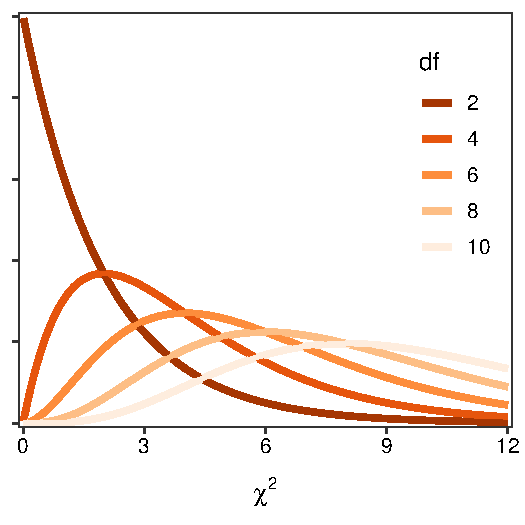
\includegraphics[width=.4\linewidth]{Figs/chiDist-1} 

}

\caption[$\chi^2$ distributions with varying degrees-of-freedom]{$\chi^2$ distributions with varying degrees-of-freedom.}\label{fig:chiDist}
\end{figure}


\end{knitrout}

Unlike the normal and t distributions, the $\chi^2$ distribution always represents the two-tailed situation, although the ``two tails'' will appear as one tail on the right side of the distribution. The simplest explanation for this characteristic is that the ``squaring'' in the calculation of the $\chi^{2}$ test statistic results in what would be a ``negative tail'' being ``folded over'' onto what is the ``positive tail.''  Thus, all probability (i.e., area) calculations on a $\chi^{2}$ distribution represent the two-tailed alternative hypotheses.

Proportional areas on a $\chi^2$ distribution are computed with \R{disrib()}. The major differences with a $\chi^2$ distribution is that \R{distrib="chisq"} must be used in \R{distrib()} and the degrees-of-freedom must be given to \R{df=} (how to find the df will be discussed in subsequent sections). In addition, \R{lower.tail=FALSE} is always used when computing a p-value because the upper-tail probability represents the two-tailed alternative hypothesis inherent to all Chi-Square Tests. For example, the area right of $\chi^2=6.456$ on a $\chi^2$ distribution with 2 df is 0.0396 \figrefp{fig:chiarea1}.
\vspace{-3pt}
\begin{knitrout}
\definecolor{shadecolor}{rgb}{0.922, 0.922, 0.922}\color{fgcolor}\begin{kframe}
\begin{verbatim}
> ( distrib(6.456,distrib="chisq",df=2,lower.tail=FALSE) )
[1] 0.03963669
\end{verbatim}
\end{kframe}\begin{figure}[hbtp]

{\centering 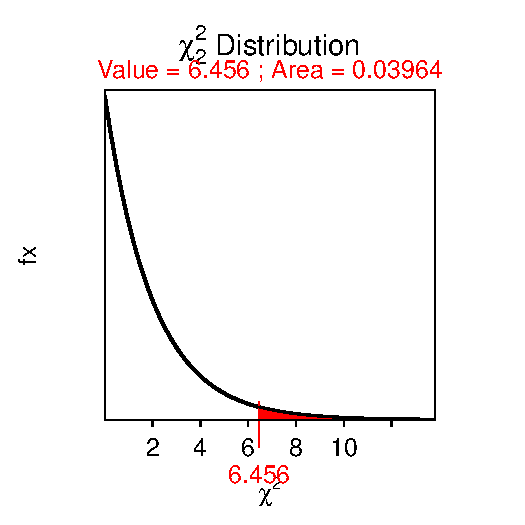
\includegraphics[width=.4\linewidth]{Figs/chiarea1-1} 

}

\caption[Depiction of the area to the right of $\chi^2=6.456$ on a $\chi^2$ distribution with 2 df]{Depiction of the area to the right of $\chi^2=6.456$ on a $\chi^2$ distribution with 2 df.}\label{fig:chiarea1}
\end{figure}


\end{knitrout}


\section{Chi-Square Test Specifics}
\vspace{-3pt}
Researchers commonly want to compare the distribution of individuals into the levels of a categorical variable among two or more groups (or populations). For example, researchers may want to determine if the disribution of failing students differs between males and females, if the distribution of kids playing sports differs between kids from high- or low-income families, if the distribution of four major plant species differs between two locations, or if the distribution of responses to a five-choice question differs between respondents from neighboring counties. All of these questions have a categorical response variable (fail or not, play sport or not, plant species, answer to five-choice question) compared among two or more groups (gender, income category, two locations, neighboring counties). The Chi-Square Test, the subject of this module, can be used for each of these situations.\footnote{The Chi-Square Test is quite flexible and can be derived from different types of hypotheses than those described here.}

\subsection{Hypotheses}
\vspace{-3pt}
The statistical hypotheses for a Chi-Square Test are ``wordy.''  To explore this, let's first assume that a two-way frequency table (see \modref{chap:BivEDACat}) will summarize the data where the rows correspond to separate groups and the columns correspond to levels of the response variable. In this organization, the Chi-Square Test null hypothesis is that the row percentages are equal -- i.e., ``the percentage distribution of individuals into the levels of the response variable is the same for all groups.''  The alternative hypothesis states that there is some difference among the row percentages -- i.e., ``the percentage distribution of individuals into the levels of the response variable is NOT the same for all groups.''

As one example (more are shown below), consider the following:
\vspace{-6pt}
\begin{quote}
\textsl{An association of Christmas tree growers in Indiana sponsored a survey of Indiana households to help improve the marketing of Christmas trees. Of the 261 rural households, 64 had a natural tree (as compared to an artificial tree). Of the 160 urban households, 89 had a natural tree. Use these results to determine, at the 10\% level, if the distribution of households with a natural tree differed between rural and urban households.}
\end{quote}
\vspace{-3pt}

The hypotheses for this situation are,
\[ \begin{split}
  H_{0}&: \text{``the distrubution of households into the tree types is the same for urban and rural households''} \\
  H_{A}&: \text{``the distrubution of households into the tree types is NOT the same for urban and rural households''}
\end{split} \]


\subsection{Tables}
\vspace{-6pt}
As noted above, all two-way frequency tables used for a Chi-Square Test will be organized such that the response variable forms the columns and the groups to be compared form the rows. With this organization, the row-percentage table becomes the table of primary interest because it relates directly to the hypotheses described above. The question of a Chi-Square Test then becomes one of determining whether each row of the row-percentage table is equal, given sampling variability.

The observed raw data must be organized into a two-way frequency table as described in \modref{chap:BivEDACat}. For example, the Christmas tree data is summarized as in \tabref{tab:ChiTreeObs}. The actual calculations for a Chi-Square Test are performed on this observed table. However, the hypothesis test, as described above, is best viewed as a method to determine if each row of the row-percentage table is statistically equivalent or not. Thus, the row-percentage table computed from the frequency table is useful when interpreting the results of a Chi-Square Test \tabrefp{tab:ChiTreeObsProp}.

\begin{table}[htbp]
  \centering
  \caption{Frequency of individuals in urban and rural households that have a natural or an artificial Christmas tree.}\label{tab:ChiTreeObs}
    \begin{tabular}{c|c|c|c|}
      \multicolumn{1}{c}{} & \multicolumn{2}{c}{Tree Type} & \multicolumn{1}{c}{} \\
      \cline{2-3}
      Household & Natural & Artificial & \multicolumn{1}{c}{} \\
      \hline
      \multicolumn{1}{|c|}{Urban} & 89 & 172 & \textbf{261} \\
      \hline
      \multicolumn{1}{|c|}{Rural} & 64 & 96 & \textbf{160} \\
      \hline
       & \textbf{153} & \textbf{268} & \textbf{421} \\
      \cline{2-4}
    \end{tabular}
\end{table}

\begin{table}[htbp]
  \centering
  \caption{Percentage of individuals within urban and rural households that have a natural or an artificial Christmas tree.}\label{tab:ChiTreeObsProp}
    \begin{tabular}{c|c|c|c|}
      \multicolumn{1}{c}{} & \multicolumn{2}{c}{Tree Type} & \multicolumn{1}{c}{} \\
      \cline{2-3}
      Household & Natural & Artificial & \multicolumn{1}{c}{} \\
      \hline
      \multicolumn{1}{|c|}{Urban} & 34.1 & 65.9 & \textbf{100.0} \\
      \hline
      \multicolumn{1}{|c|}{Rural} & 40.0 & 60.0 & \textbf{100.0} \\
      \hline
       & \textbf{36.3} & \textbf{63.7} & \textbf{100.0} \\
      \cline{2-4}
    \end{tabular}
\end{table}

The Chi-Square Test requires constructing a table of expected values that are derived from the null hypothesis. Specifically, the ``expected'' table contains the expected frequency of individuals in each level of the response variable for each group assuming that the distribution of responses does not differ among groups. These expected tables are computed from the margins of the observed table, but are best explained with an illustrative example.

In the Christmas tree example, the null hypothesis states that there is no difference in the distribution of households with a natural tree between the rural and urban areas. Thus, under this null hypothesis, one would expect the proportion (or percentage) of households with a natural tree to be the same in both groups. The proportion of households with a natural tree, regardless of location, is $\frac{153}{421}$=$0.363$. Thus, under the null hypothesis, the proportion of rural AND the proportion of urban households with a natural tree is $0.363$. Because there is a different number of urban and rural households in the study, the actual NUMBER (rather than proportion) of households expected to have a natural tree will differ. The NUMBER of urban households expected to HAVE a natural tree is found by multiplying the number of urban households by the common proportion computed above -- i.e., $261*0.363$=$94.743$. The remaining urban households would be expected to NOT have a natural tree -- i.e., $261-94.743$=$261(1-0.363)$=$166.257$. Similar calculations are made for the rural households (i.e., $160*0.363=58.080$ expected to have a natural tree and $160*(1-0.363)=101.920$ expected to NOT have a natural tree.

These expected frequencies are computed directly and easily from the marginal totals of the observed frequency table \tabrefp{tab:ChiTreeObs}. For example, substituting the fractional representation of the decimal proportions into the calculation of the expected number of urban households with a natural tree gives $261*\frac{153}{421}$=$\frac{261*153}{421}$=$94.853$\footnote{Note a slight difference here because 0.363 was rounded to three decimals, whereas the fraction is not rounded.}. A close examination of this formula and the marginal totals in \tabref{tab:ChiTreeObs} shows that this value is equal to the product of the corresponding row and column marginal totals in the observed table divided by the total number of individuals. The other expected values follow a similar pattern as follows,
\begin{Itemize}
  \item $261*\frac{268}{421}=\frac{261*268}{421}=166.147$ urban households to NOT have a natural tree.
  \item $160*\frac{153}{421}=\frac{160*153}{421}=58.147$ rural households to have a natural tree.
  \item $160*\frac{268}{421}=\frac{160*268}{421}=101.853$ rural households to NOT have a natural tree.
\end{Itemize}

Thus, all expected values in a Chi-Square Test are calculated by multiplying the row and column totals of the frequency table and dividing by the total number of individuals. These expected values are summarized in a two-way table, called the expected frequencies table \tabrefp{tab:ChiTreeExp}.

\begin{table}[htbp]
  \centering
  \caption{The expected frequency of individuals in urban and rural households that have a natural or an artificial Christmas tree.}\label{tab:ChiTreeExp}
    \begin{tabular}{c|c|c|c|}
      \multicolumn{1}{c}{} & \multicolumn{2}{c}{Tree Type} & \multicolumn{1}{c}{} \\
      \cline{2-3}
      Household & Natural & Artificial & \multicolumn{1}{c}{} \\
      \hline
      \multicolumn{1}{|c|}{Urban} & 94.853 & 166.147 & \textbf{261} \\
      \hline
      \multicolumn{1}{|c|}{Rural} & 58.147 & 101.853 & \textbf{160} \\
      \hline
       & \textbf{153} & \textbf{268} & \textbf{421} \\
      \cline{2-4}
    \end{tabular}
\end{table}

\subsection{Specifics}
\vspace{-3pt}
The Chi-Square Test is characterized by a categorical response variable recorded for two or more groups (or populations). The specifics of the Chi-Square Test are in \tabref{tab:Chispec}.

\begin{table}[h]
\centering
\colorbox{ltgray}{
\begin{minipage}{.8\textwidth}
  \centering
	\caption{Characteristics of a Chi-Square Test.}\label{tab:Chispec}
\vspace{-3pt}
  \begin{Itemize}
      \item \textbf{Null Hypothesis:} ``The distribution of individuals into the levels of the response variable is the same for all groups''
      \item \textbf{Alternative Hypothesis:} ``The distribution of individuals into the levels of the response variable is NOT the same for all groups.''
      \item \textbf{Statistic:} Observed frequency table.
      \item \textbf{Test Statistic:} $\chi^{2} = \Sum_{cells}\frac{(Observed-Expected)^{2}}{Expected}$
      \item \textbf{df:} $(r-1)(c-1)$ where $r=$ number of rows and $c=$ number of columns
      \item \textbf{Assumptions:} Expected value for each category is $\geq5$.
      \item \textbf{Use with:} Categorical response, two or more groups (or populations).
  \end{Itemize}
\end{minipage}}
\end{table}

A confidence region is not usually constructed for a Chi-Square Test because of the complexity of the statistics and parameter. Thus, Step 11 for a hypothesis test will not be computed for a Chi-Square Test.

\vspace{-6pt}
\subsection{Example -- Christmas Trees}
\vspace{-6pt}
Below are the 11-steps \sectrefp{sec:11Steps} for a full hypothesis test for the Christmas tree example.
\vspace{-10pt}
\begin{Enumerate}
  \item $\alpha$=0.10.
  \item $H_{0}$: ``distribution of households by type of tree is the same for urban and rural households'' vs. $H_{A}$: ``distribution of households by type of tree is NOT the same for urban and rural households.''
  \item A Chi-Square Test is required because (i) a categorical response variable was recorded (type of tree) and (ii) two groups are being compared (urban and rural households).
  \item The data appear to be part of an observational study with no clear indication of randomization.
  \item The expected frequency in each of the four cells is greater than five \tabrefp{tab:ChiTreeExp}.
  \item The observed frequency table is in \tabref{tab:ChiTreeObs}.
  \item $\chi^{2}$ = $\frac{(89-94.853)^{2}}{94.853}$ + $\frac{(172-166.147)^{2}}{166.147}$ + $\frac{(64-58.147)^{2}}{58.147}$ + $\frac{(96-101.853)^{2}}{101.853}$ = $0.3611+0.2062+0.5891+0.3363$ = $1.4927$ with 1 df.
  \item p-value=$0.2218$.
  \item $H_{0}$ is not rejected because the p-value is $>\alpha$.
  \item There does not appear to be a significant difference in the distribution of Christmas tree types among rural and urban households.
  \item Not performed for Chi-Square Test.
\end{Enumerate}

\vspace{-6pt}
\begin{minipage}{\textwidth}
\textbf{R Appendix:}
\vspace{-6pt}
\begin{knitrout}
\definecolor{shadecolor}{rgb}{0.922, 0.922, 0.922}\color{fgcolor}\begin{kframe}
\begin{verbatim}
( distrib(1.4927,distrib="chisq",df=1,lower.tail=FALSE) )
\end{verbatim}
\end{kframe}
\end{knitrout}
\end{minipage}



%    \cleardoublepage
%    \phantomsection
%    \addcontentsline{toc}{part}{Appendix}
%    \chapter*{Appendices}
%    \appendix


%  \backmatter
%    %BIBLIOGRAPHY ---------------------------------------------------------------------------------------------------------
\cleardoublepage                             %not sure why but this is needed so TOC entry will point to right start page
\phantomsection                              %not sure why but this is needed so TOC entry will point to right start page
\addcontentsline{toc}{part}{Bibliography}    %Add a TOC entry
\bibliography{c:/aaaWork/zGnrlLatex/DHO_Bib} %make the bibliography
 
%INDEX ----------------------------------------------------------------------------------------------------------------
% cross references for the index
\index{Alternative Hypothesis|see{Hypothesis, Alternative}}
\index{Coefficient of Determination|see{$r^{2}$}}
\index{Forward calculation|see{Normal Distribution, Finding areas}}
\index{Frequency Table|see{Table, Frequency}}
\index{Goodness-of-Fit Test|see{Chi-square}}
\index{Line!Finding best-fit|see{Regression}}
\index{Mean!Inference|see{Z-test and t-Test}}
\index{Null Hypothesis|see{Hypothesis, Null}}
\index{Percentage Table|see{Table}}
\index{Proportions Table|see{Table, Proportion}}
\index{Row Proportions Table|see{Table, Proportion}}
\index{Column Proportions Table|see{Table, Proportion}}
\index{Table Proportions Table|see{Table, Proportion}}
\index{Proportions, Inference|see{Chi-square}}
\index{Rejection Criterion|see{$\alpha$}}
\index{Reverse calculation|see{Normal Distribution, Finding values}}
\index{Simple Linear Regression|see{Regression}}
\index{SLR|see{Regression}}
\index{Standard Normal Distribution|see{Normal Distribution}}
\index{Standardization|see{Normal Distribution, Converting to Z-scale}}
\index{One-sample Z-Test|see{Z-Test}}
\index{1-sample Z-Test|see{Z-Test}}
\index{One-sample t-Test|see{t-Test}}
\index{1-sample t-Test|see{t-Test}}
\index{Two-sample t-Test|see{t-Test}}
\index{2-sample t-Test|see{t-Test}}
\index{Matched-Pairs t-Test|see{t-Test}}
\index{Two-way Table|see{Table, Frequency}}
\index{Type I Error|see{Hypothesis Testing, Errors}}
\index{Type II Error|see{Hypothesis Testing, Errors}}
\index{Variability!Natural|see{Natural Variability}}
\index{Variability!Sampling|see{Sampling Variability}}
\index{Variable!Types|see{Quantitative, Continuous, Discrete, Categorical, Nominal, or Ordinal}}
\index{Variance!Testing Equality|see{Levene's Test}}
\index{Y-intercept|see{Intercept}}
\index{Z-Distribution|see{Normal Distribution, Standard Normal}}

% code to actually add the index
\addtocontents{toc}{\setlength{\cftbeforepartskip}{0.4em}}  %decrease dist before parts in back matter portion of TOC
\cleardoublepage                          %not sure why but this is needed so TOC entry will point to right start page
\phantomsection                           %not sure why but this is needed so TOC entry will point to right start page
\addcontentsline{toc}{part}{Index}        %Add a TOC entry
\printindex                               %Make the index


\end{document}
